\documentclass[12pt,english,hyperfootnotes=false,hidelinks]{article}

%%%% Packages
\usepackage{lmodern}
\usepackage{tablefootnote}
\usepackage[T1]{fontenc}
\usepackage[latin9]{inputenc}
\usepackage{geometry}
\geometry{verbose,tmargin=1.25in,bmargin=1.25in,lmargin=1.25in,rmargin=1.25in}
\usepackage{float}
\usepackage{enumitem}
\usepackage{amsmath}
\usepackage{graphicx}
\usepackage{setspace}
\usepackage[authoryear]{natbib}
\usepackage[bottom,multiple]{footmisc}
\usepackage{geometry}
\usepackage{adjustbox}
\usepackage[hyphenbreaks]{breakurl}
\usepackage{booktabs}
\usepackage{pdflscape}
\usepackage{siunitx}
\usepackage{numprint}
\usepackage{threeparttable}
\usepackage{caption}
\usepackage{babel}
\usepackage{xcolor}
\usepackage{longtable}
\usepackage{afterpage}
\usepackage{dcolumn}
\usepackage{multicol}
\usepackage{amsfonts}
\usepackage{adjustbox}
\usepackage{xurl}
\usepackage{hyperref}
\usepackage{catchfilebetweentags}
\usepackage{csquotes}
\usepackage{framed}
\usepackage{multirow}
\usepackage{tikz}
\usetikzlibrary{decorations.pathreplacing}
\usepackage{makecell}
\usepackage{natbib}
% define check and xmark
\usepackage{pifont}
\newcommand{\cmark}{\ding{51}}%
\newcommand{\xmark}{\ding{55}}%

%%%% Other settings
\captionsetup[table]{skip=0pt}
\interfootnotelinepenalty=10000
\newcolumntype{R}[1]{>{\raggedright\let\newline\\\arraybackslash\hspace{0pt}}m{#1}}
\newcolumntype{C}[1]{>{\centering\arraybackslash}m{#1}}

\newtheorem{assumption}{Assumption}

%%% Command for extracting numbers
\newcommand{\gn}[1]{\ExecuteMetaData[results/results.tex]{#1}}



\title{
Bureaucratic Capacity and Urban Planning: Evidence from Los Angeles
\thanks{
This project was supported in part by the UCLA Ziman Center for Real Estate Research. We thank the Ziman Center for its financial support. We also thank Ignacio Ramirez for his invaluable research assistance. The views expressed in this paper are solely those of the authors and do not necessarily reflect those of the Ziman Center. All errors are our own.
}
}

\author{
    Stuart Gabriel\thanks{UCLA Anderson School of Management, 110 Westwood Plaza, Suite C412, Los Angeles, CA 90095-1481;  stuart.gabriel@anderson.ucla.edu} \and
    M.J. Histen\thanks{California State University, Northridge, David Nazarian College of Business and Economics, 18111 Nordhoff St, Northridge, CA 91330; matthew.histen@csun.edu} \and
    Edward Kung\thanks{Corresponding Author: California State University, Northridge, David Nazarian College of Business and Economics, 18111 Nordoff St, Northridge, CA 91330; edward.kung@csun.edu}
}

\date{\today}

\begin{document}

\maketitle

\singlespacing

\vspace{-1cm}

\begin{abstract}
Using data from the Los Angeles City Planning Commission, we document the role of bureaucratic capacity in influencing urban development outcomes. We show public opposition and familiarity of cases matter. Cases that are fairly typical are more likely to sail through approvals, but cases exhibiting peculiar features are less likely to be approved and more likely to be delayed. We measure familiarity by how semantically unique the proposal is to other proposals of its category. A one standard deviation increase in uniqueness decreases the log odds of approval by \gn{SemUniCoef}. Public opposition matters as well: a doubling of the number of opposition letters reduces the log odds of approval by \gn{NOppCoef}. The results are consistent with a model of bureaucratic choice with public monitoring, reputational risk, and cognitive constraints.
\end{abstract}


\noindent{\textit{Keywords}: local land-use regulation, bureaucratic efficiency} \\
\noindent {\textit{JEL} Classification: D73, R14, R38, R52.} \\


\doublespacing

\pagebreak

%\section{Introduction}\label{sec_intro}

There is growing recognition among researchers, policymakers, and even popular media that stringent land use regulations are contributing to reduced housing production and high housing costs in America and much of the Western world.\footnote{\citet{klein2025abundance} have recently brought the issue to popular attention in their book \emph{Abundance}.} In the urban economics literature, many papers have demonstrated a link between land use regulations and housing market outcomes. For example, \citet{ganongshoag2017} showed how rising house prices are correlated with housing supply regulations, and may have explained regional income divergence in the U.S. in recent decades. \citet{brueckner2020} showed how building heights in many U.S. cities are below competitive equilibrium levels due to floor-area-ratio restrictions. Similar findings have been demonstrated in different geographic markets: \citet{glaeser2009} in Boston, \citet{jackson2016} for California cities, \citet{hilber2016} in England. There are many more, more than can be listed here, and we direct the reader to \citet{gyourkomolloy2015} and \citet{molloy2020} for further review. In addition to the empirical effects of housing supply regulation on housing outcomes, a number of papers have argued that these effects can lead to spatial misallocation of resources \citep{turner2014, albouy2018, hsieh2019, gabriel2020}. 

Despite the growing understanding of the impact of land use regulations, still little is known about the regulatory production function itself. That is, we know that land use regulations affect outcomes---but how are the regulations produced and how are they enforced? And does the regulatory \emph{process} itself meaningfully impact outcomes over and above the \emph{de jure} text of the regulations? For example, regulations say what can be built, where, but often allow for exceptions. Even if exceptions are ultimately always granted, does limited capacity for processing exceptions impact housing outcomes? It seems likely that the answer is yes, as \citet{gabrielkung2025} showed that long bureaucratic approval times can significantly reduce to the rate of housing production. Yet, little is known about the role of bureaucratic capacity or its determinants.

This paper aims to fill that gap by providing empirical evidence for the role of bureaucratic capacity in the housing production process. We use data from the proceedings of the Los Angeles City Planning Commission (LA CPC). The LA CPC is a nine member administrative body with members appointed by the Mayor of LA and confirmed by the City Council. The CPC is responsible for reviewing zoning changes, approving conditional use permits for large developments, and handling appeals of decisions made by lower bodies. Decisions of the CPC are made by majority rule. The agenda for each meeting is set by the Commission itself and made available to the public at least 7 days before the meeting. The minutes of each meeting are also published online. The minutes record the order of discussion, the motions made on each agenda item, and the votes made on each motion. In addition, members of the public are allowed to submit comments on any agenda items either in writing or in person during the meeting.

The agenda, minutes, and written public comments of each CPC meeting are all made available to the public by the City of Los Angeles. We use this data to investigate the determinants of CPC decision making. We find that the CPC is responsive to public opinion: greater public opposition to a project makes it less likely to be approved, and more likely to get denied, delayed, or to have conditions attached to the approval. In addition, we find that unusual projects, as measured by their semantic dissimilarity to other requests, are also more likely to be denied, delayed, or to have conditions attached to the approval. This suggests that bounded rationality may play a role in the approvals process: projects that are unfamiliar and fall outside of normal routines require more cognitive load from the Commission, and are thus less likely to pass through smoothly. The statistical relationship between case approval and semantic uniqueness survives even after controlling for potential confounding factors, such as the types of requests made in the proposal and the overall complexity of the proposal. Lastly, we find that the CPC uses a procedural tool known as a ``Consent Calendar'' to streamline approvals for routine and non-controversial items, further consistent with the hypothesis that cognitive capacity is an important input in the CPC's bureaucratic decision-making.

To our knowledge, this is the first paper to provide direct empirical evidence of the bureaucratic inputs to the land use regulatory process. We demonstrate that public opposition and cognitive capacity are both significant drivers of LA CPC decision-making. Although we do not quantify the impact of these factors on aggregate housing supply, the results do suggest that reducing regulatory complexity and streamlining the regulatory process could lead to a meaningful acceleration of housing production. The results also contribute to the broader literature on bureaucratic decision-making and bounded rationality, which we discuss further in Section \ref{sec_model}.

The rest of the paper is organized as follows. Section \ref{sec_model} discusses the literature on bureaucratic decision-making and develops a simple model of CPC decision-making that can rationalize our empirical results. Section \ref{sec_data} describes how we collected and processed the data. Section \ref{sec_methodology} describes the empirical methodology and section \ref{sec_results} presents the results. Section \ref{sec_conclusion} concludes.




\section{Introduction}\label{sec_intro}

Since \citet{Simon1955}, the concept of bounded rationality has reshaped how we understand decision-making. Rather than assuming fully informed optimization, actors operate with limited attention, information, and computational capacity. Most decisions---indeed, most organizational arrangements---exist precisely to manage these limits. For an organization or a policy to function, it must economize on information, distributing attention and routinizing choice across actors \citep{CyertMarch1963}. Rules, hierarchies, and standards function as compression devices that simplify complexity so boundedly rational agents can act. Institutional design, in this sense, involves a trade-off: reducing informational complexity makes collective action possible, but oversimplification can constrain discretion and innovation.

Still, Simon's insight is more descriptive than operational. His original formulation was broad, leaving open what it means to ``satisfice'' or how cognitive constraints work in practice. Subsequent research has attempted to formalize bounded rationality through explicit limits on optimization or information processing. In one branch, agents are modeled as satisficers, engaging in constrained search over feasible options \citep{Stigler1961,Rubinstein1986,Salant2011}. Another tradition treats cognition as a scarce resource allocated across noisy or incomplete signals \citep{Radner1993,VanZandt1999,Sims2003}. More recent approaches impose restrictions on reasoning itself. Agents cannot process all states or clauses within a choice architecture and therefore use simplified mental representations \citep{ZhangLevin2017,Jakobsen2020}. Simulation studies extend these ideas to dynamic settings, showing that when decision-makers can only make local, incremental improvements \citep{Levinthal1997,MarengoDosi2005,Richters2021}, outcomes depend as much on the structure of the decision landscape as on individual preferences or rules.

These theoretical advances have added clarity, but translating them into empirical work remains challenging. Because cognitive limits are inherently unobservable, they can only be inferred indirectly through deviations from idealized rationality. Behavioral economists have modeled this process as probabilistic optimization, where agents make noisy or limited best responses \citep{McKelveyPalfrey1995,CamererHoChong2004}. Experimental studies have documented satisficing and cognitive constraints \citep{Guth2010,LimMatrosTurocy2014,AlaouiJanezicPenta2020}, but remain confined to stylized laboratory environments. Systematic evidence from field settings is scarce \citep{Kirman2010,FehrSchmidt1999}, leaving open how bounded rationality operates in practice. As a result, the empirical literature lacks large-scale, observational analyses that trace how cognitive constraints manifest in organizational decision environments.

This paper addresses that gap. We study bounded rationality in the empirical setting of the Los Angeles City Planning Commission (LACPC), an administrative body that decides which development projects proceed in the city. Commissioners evaluate proposals that combine legal, architectural, and community considerations under tight time limits and public scrutiny. Each case requires filtering substantial information while balancing political and legal considerations. The public nature of the process generates a rich paper trail: every meeting produces agendas, minutes, and written comments that record both the information presented and the decisions made. We use these records to construct a measure of semantic uniqueness by converting the text into high-dimensional vector embeddings. Cases that use similar language cluster together, and a proposal's uniqueness is defined by how far it lies from the center of its cluster. Projects with greater semantic distance impose higher cognitive effort, as commissioners must interpret unfamiliar items.

At its core, the Commission's task reflects a classic principal-agent problem. Commissioners act as agents on behalf of the city, charged with advancing development while ensuring compliance with zoning rules and public expectations. For each proposal, commissioners decide whether to delay, modify, or approve a project, subject to two constraints. First, they face oversight risk: every decision is publicly scrutinized by residents, community organizations, and the press. Excessive leniency or excessive postponements can cause political backlash. We capture this dimension by applying sentiment analysis to public correspondence as an indicator of monitoring pressure. Second, commissioners face cognitive limits: each meeting includes dozens of cases that vary in legal and technical complexity. We proxy for the cognitive effort in interpreting proposals using semantic uniqueness, which measures how linguistically similar each proposal is relative to the kinds of cases the Commission typically encounters. 

We use this framework to estimate how cognitive limits and public oversight correspond to approval outcomes using an ordered logit specification. The results reveal a consistent pattern. Less familiar projects face a penalty: controlling for project type, council district, and case characteristics, a one-standard-deviation increase in semantic uniqueness reduces the odds of full approval by about \gn{SemUniCoefPct} percent. Routine items, by contrast, move easily through the process. Placement on the Commission's consent calendar, which groups standard cases for joint approval, nearly doubles the probability of full approval. Public opposition exerts a similarly strong negative effect, while support provides little offsetting benefit. Doubling the number of opposition letters lowers the likelihood of approval by roughly the same magnitude as an equivalent increase in semantic uniqueness.

These dynamics are particularly consequential in the context of urban development, where regulatory decisions directly shape the pace and composition of housing supply. A large literature has shown that stringent land-use regulations constrain construction and contribute to high housing costs.\footnote{See, for example, 
\citet{glaeser2009},
\citet{hilber2016},
\citet{ganongshoag2017},
\citet{brueckner2020},
and \citet{gabrielkung2025}.
See \citet{gyourkomolloy2015} and \citet{molloy2020} 
for further reviews of the literature.} 
Yet much less is known about the \emph{regulatory production process} itself---how administrative capacity, attention, and procedural design influence which projects advance and which stall. By showing that cognitive and oversight constraints systematically affect approval outcomes, our analysis provides evidence on a key mechanism linking bureaucratic performance to housing supply.

Our study contributes to two related areas of research. First, the paper provides an empirical grounding for the theory of bounded rationality by documenting cognitive constraints in real organizational settings. Using policy documents, we extract and quantify information to capture latent cognitive dimensions such as familiarity, complexity, and attention. In doing so, the paper offers a general framework for quantifying the cognitive costs of decision-making, which can be applied across institutional contexts to examine how information-processing limits shape organizational behavior. Second, it extends models of bureaucratic behavior by treating regulatory outcomes as functions of cognitive capacities as well as incentives. Whereas prior work has focused on malformed incentives or political capture (e.g., \citealp{Prendergast2003}; \citealp{CarpenterKrause2012}; \citealp{BusuiocLodge2016}), our results show that even in the absence of explicit bias, limited processing capacity can produce variation in outcomes. The analysis further contributes to the literature on urban regulation and housing supply (e.g., \citealp{gyourkomolloy2015}; \citealp{molloy2020}) by suggesting that the pace of development depends not only on statutory constraints but also on the institutional capacities of the regulatory apparatus itself.

The remainder of the paper is organized as follows. Section \ref{sec_model} situates our analysis within the literature on bureaucratic decision-making and develops a simple model that formalizes the trade-off between oversight risk and cognitive cost. Section \ref{sec_data} describes the Los Angeles City Planning Commission and the construction of the text-based dataset. Section \ref{sec_methodology} outlines our empirical methodology and variables, including the computation of semantic uniqueness. Section \ref{sec_results} presents the main results and robustness checks, and Section \ref{sec_conclusion} concludes.
\section{A Basic Model} \label{sec_model}

Two recurring constraints arise in bureaucratic decision-making: reputational risks under public oversight and cognitive limits in processing complex proposals. We review these institutional features of the decision environment, then present a simple model in which commissioners choose actions and effort under both constraints. The model shows how these trade-offs generate a systematic bias against unfamiliar or contested projects, while routine items sail through with little resistance.

\subsection{Oversight, Cognition, and Bureaucratic Choice}

Bureaucratic decision-making is shaped by the limited contractibility and imperfect measurability of tasks, which create persistent incentive problems \citep{Dixit2002}. Public officials therefore operate under binding institutional and cognitive constraints that systematically shape their choices.

One constraint arises from the cost of oversight. Establishing and operating monitoring institutions is expensive \citep{HuberShipan2000,DamonteDunlopRadaelli2014}. Consequently, oversight depends on indirect signals. Since the public cannot directly observe bureaucratic effort or expertise, it relies on ``fire alarms'' such as complaints or organized opposition \citep{Prendergast2003}. Such monitoring is asymmetric: failures generate complaints, while successes rarely do. This asymmetry makes bureaucrats rationally defensive, leading them to minimize exposure by avoiding novel or controversial decisions. Moreover, accountability is rarely unitary. Agencies are monitored by legislators, courts, media, and citizens, whose expectations are often incompatible \citep{Black2008,MaggettiPapadopoulos2018}. Such polycentric accountability multiplies reputational risks and encourages defensive choices over efficiency \citep{CarpenterKrause2012,GiladMaorBloom2015,BusuiocLodge2016}. Opposition letters, in this sense, are not merely signals of constituent concern but reputational threats.

A second constraint arises from the internal limits of decision-makers. Rational inattention models \citep{HebertWoodford2023} and bounded rationality frameworks \citep{deClippelRozen2021} show that officials cannot fully process all information and must selectively allocate scarce attention \citep{BesleyGhatak2003}. Unfamiliar proposals therefore impose higher cognitive costs and are more likely to be screened out \citep{DeFrancescoRadaelliTroeger2012}. Choice overload and satisficing push bureaucrats toward routine or standardized options. Goal ambiguity further complicates evaluation: when standards are unclear, performance falls and risk aversion rises \citep{AndersonStritch2016}. In such settings, the safest course is to stress procedural appropriateness or technical diligence, often at the expense of innovation \citep{Gilad2015,Duvanova2012}.

Because the risks are concentrated while the benefits are diffuse, bureaucrats are incentivized to delay or modify proposals even when those projects may generate social value. The result is a systematic bias: safe, routine projects advance, while novel or contested ones are sidelined regardless of their potential.


\subsection{Model}

Each commissioner chooses an action $a \in \{0,1,2\}$, where $a=0$ denotes delay, $a=1$ denotes modification, and $a=2$ denotes full approval. The commissioner may 
also exert effort $e \geq 0$, representing the diligence devoted to evaluating and justifying a project. Effort simultaneously increases the cognitive burden of processing unfamiliar projects and decreases the expected penalties from oversight.

Two observable project attributes matter:

\begin{itemize}
    \item \textbf{Unfamiliarity} $\delta \geq 0$: Low values correspond to routine, standardized projects; high values correspond to unusual, novel, or hard to evaluate proposals.
    \item \textbf{Opposition} $\chi \geq 0$: The volume of opposition letters received, which increases the salience of oversight.
\end{itemize}

The commissioner's utility is
\begin{equation}
    U_A(a,e,\delta,\chi) \;=\; B(a) \;-\; C(e,\delta) \;-\; M(a,e,\chi)
    \label{eq:agentutility}
\end{equation}
where:
\begin{itemize}
    \item $B(a)$ is the baseline benefit from taking action $a$. These benefits can be interpreted broadly, but in general, approving projects creates visible productivity. We assume $B(2)\geq B(1)\geq B(0)$, so that in the absence of processing costs or oversight risk the commissioner would prefer more approvals.
    \item $C(e,\delta)$ is the information-processing cost, increasing in both unfamiliarity ($C_\delta >0$). This term captures the cognitive demands of evaluating non-routine projects. As unfamiliarity $\delta$ rises, commissioners face greater goal ambiguity (unclear standards for what counts as an acceptable project) and bounded rationality constraints (limited attention to fully process all pieces of the project). 
    \item $M(a,e,\chi)$ is the monitoring penalty function from the reputational, political, or legal cost associated with taking action $a$ with effort $e$ when opposition intensity is $\chi$. It is increasing in approval intensity ($M_a > 0$) and in opposition ($M_\chi > 0$), but decreasing in effort ($M_e < 0$). Decreasing in $e$ reflects the idea that additional due diligence makes decisions more defensible under scrutiny, thereby reducing expected penalties.
\end{itemize}

For any given action $a$, the commissioner chooses optimal effort $e^*$ satisfying the first-order condition
\begin{equation}
    C_{e}(e^*,\delta) \;=\; -\, M_{e}(a,e^*,\chi).
    \label{eq:effortFOC}
\end{equation}
The commissioner chooses effort so that the marginal cost of diligence offsets the marginal reduction in expected monitoring penalties. Greater unfamiliarity raises the burden of processing, while higher levels of opposition increase the salience of oversight.

To capture the joint choice of action and effort, we impose a mild regularity so that monitoring responds in the intuitive way, where stronger approval requires greater diligence under scrutiny, and opposition makes diligence more consequential by increasing how much it reduces expected penalties. Formally, the restrictions
\[
\begin{aligned}
M_{ea}(a,e,\chi) &< 0 \\
M_{e\chi}(a,e,\chi) &< 0 \\
C_{e\delta}(e,\delta) &> 0
\end{aligned}
\]
imply that optimal effort responds monotonically: $e^*$ increases in action $a$ and opposition $\chi$, but decreases in unfamiliarity $\delta$. This means that approving a contested project requires additional diligence to limit expected penalties, while unfamiliar projects make each unit of diligence more costly. After selecting the optimal effort $e^*$, the commissioner then chooses the action $a$ that maximizes $U_A^*$, evaluating processing costs and monitoring penalties at $e^*$.

\subsection{Comparative Statics}

We derive three simple predictions.\\


\textbf{Proposition 1.} \textit{Opposition reduces approvals.}\\

Higher opposition $\chi$ reduces the probability that the commissioner chooses full approval. Since $M_\chi > 0$, greater opposition raises the expected monitoring penalty $M(a,e,\chi)$, reflecting the heightened likelihood of ex post scrutiny. Commissioners can respond by increasing effort to reduce these penalties, but additional diligence is costly and cannot fully neutralize political or reputational blowback. As a result, when opposition is substantial, the safer course is to shift toward modification or delay rather than approve a contested project.\\

\textbf{Proposition 2.} \textit{Unfamiliarity reduces approvals.}\\

Holding opposition $\chi$ fixed, higher unfamiliarity $\delta$ reduces the probability that the commissioner chooses full approval. Since $C_\delta > 0$, greater unfamiliarity raises the processing cost $C(e,\delta)$, making each unit of effort more expensive. Because approving an unusual project also requires more diligence to withstand scrutiny, unfamiliarity couples higher approval outcomes with prohibitively costly effort. Commissioners therefore choose modification or delay as $\delta$ rises.\\

\textbf{Proposition 3.} \textit{Consent items are more likely to be approved.}\\

Projects on the consent calendar correspond to $\delta \approx 0$, implying minimal processing costs $C(e,0)$ and low baseline monitoring penalties. Routine projects therefore require little effort to justify and face low scrutiny, making them strictly more likely to receive full approval than otherwise comparable non-consent items.\\
\section{Data}\label{sec_data}

\subsection{Institutional Background}

The Los Angeles planning and approvals process for urban development is a multi-layered process that requires the input of multiple agencies. 


\subsection{Data Acquisition}

The Los Angeles Planning Department's website maintains robust public documentation of City Planning Commission Meetings. For each meeting, the agenda, minutes, and any supplemental documents relevant to the meeting (letters from the public, traffic assessments, architectural reports, etc.) are available for download as PDF files.\footnote{As of August 26th, 2025, these documents are available at the URL: \url{https://planning.lacity.gov/about/commissions-boards-hearings}.} We downloaded these documents for all City Planning Commission meetings from May 10th, 2018 to December 19th, 2024. This resulted in documentary data for \gn{NumberOfMeetings} meetings, covering \gn{NumberOfAgendaItems} agenda items, with \gn{NumberOfSupplementalDocs} supplemental documents, spanning \gn{PageCount} pages of PDF documents. Download occurred on April 10th, 2025.

Since we are primarily interested in bureaucratic decision making, we limit our attention to the agenda items that require a decision from the board. These are identified by agenda items titled according to their Planning Department case numbers, which have a standardized format of ``[CASE PREFIX]-[YEAR]-[SERIAL NUMBER]-[CASE SUFFIXES]''. Other agenda items include items like ``Director's Report'' and ``General Public Comment'' which do not require any decisions on the part of the board. Altogether, there were \gn{NumberOfCases} agenda items requiring a decision from the board, as identified by their Planning Department case numbers.

A typical agenda item is a request from a developer to approve a development plan that goes beyond what the site's zoning designation would allow, or an appeal of a previously approved plan. Figure \ref{fig_example_agenda_item} shows an example of an agenda item. The case number is DIR-2019-6048-TOC-SPR-WDI-1A. This was a project that was initially approved by the Director of Planning (DIR). The project was granted bonuses under the Los Angeles Transit Oriented Communities program (TOC), the project requires a site plan review (SPR), and the project was granted a waiver of dedications and improvements (WDI). However, this previously approved plan was appealed (1A), and the appeal is now to be considered by the City Planning Commission. In addition to the information contained in the case number, the agenda shows additional information such as the Council District that the project is located in, and other specific details about the project proposal.

Figure \ref{fig_example_minutes_item} shows the associated minutes for the agenda item shown in Figure \ref{fig_example_agenda_item}. From the minutes, we can see that the appeal was granted in part and denied in part. The CPC upheld the Director of Planning's previous decision, but additional conditions were applied, thus allowing the project to move forward as long as the developer adheres to the new conditions. This outcome, the partial granting of an appeal or the approval of a project with modifications, is common but not the only kind of outcome. Sometimes, the requested actions by the developer are granted in their entirety without additional conditions or modifications. Rarely, the requested actions are denied entirely. A more common occurrence than denial is that the CPC puts the decision off to a later date. We will discuss the distribution of motion outcomes and voting patterns later in Section \ref{sec_descriptive_statistics}.

Figures \ref{fig_example_support_letter} and \ref{fig_example_oppose_letter} show examples of letters submitted by the public in support of and in opposition to the above project. The support letter emphasizes how the project will ease traffic, reduce air pollution, and increase housing availability. The opposition letter emphasizes concerns about displacement and how the proposed units will be unaffordable to current residents of the neighborhood. These letters typify the kinds of concern expressed by community residents in this dataset; however, the number of letters that this project attracted is atypical (DIR-2019-6048 just happens to be a particularly controversial project). We will discuss the distribution of support and opposition letters across projects later in Section \ref{sec_descriptive_statistics}.

\subsection{Data Extraction}

The documentary data provides a wealth of information about CPC cases and their outcomes. However, the information is locked within textual data that is difficult to process using traditional methods. For example, traditional NLP methods based on token and pattern matching would have a hard time comparing the agenda to the minutes and determining whether the requested actions were approved, partially approved, approved with conditions, denied, or whether the decision was postponed to a future date. 

To extract usable features from the textual content more robustly, we make use of OpenAI's \texttt{gpt-4o} generative language model. For example, the model can be asked to read the text of the agenda, read the text of the minutes, and explain what the result of committee's proposed motion was in terms of its implications for the development project---was the project approved, partially approved or approved with conditions, denied, or was the decision postponed? The methodology and prompts we used to perform the data extraction are described in detail in Appendix \ref{sec_data_appendix}. In this section, we will instead focus on the data features that were extracted from the text.

\paragraph{Agenda items.} For each agenda item, we extracted the following information from the text: 
\begin{itemize}[noitemsep, topsep=0pt]
\item Item number (used primarily for identification);
\item Item title (for cases requiring a decision, this is always a Planning Department case number)
\item Short AI-generated summary of the agenda item's content;
\item The Council District(s) to which the item applies
\end{itemize}

\paragraph{Minutes.} For each agenda item, we extract the following information from its minutes text:
\begin{itemize}[noitemsep, topsep=0pt]
\item Short AI-generated summary of the deliberations and the motion that was ultimately voted on;
\item Implication of the motion for the proposed project: were the requested actions approved, approved in part or with conditions and modifications, denied, or were deliberations continued to a future date?
\item Result of the vote (whether the motion passed or failed)\footnote{Note that a motion passing is not the same as a project getting approved, nor is a motion failing the same as a project getting denied. A Member may move to deny the project's requested actions, or move to accept an appeal of a previously approved project, in which case the motion passing implies a denial of the project. These nuances highlight why LLMs are helpful in the data extraction process.};
\item Vote tallies: the number of ayes, nays, absences, abstentions, and recusals.
\end{itemize}

\paragraph{Supplemental documents.} For each supplemental document, we extract the following information from its text:
\begin{itemize}[noitemsep, topsep=0pt]
\item Type of document: whether it is a letter or petition, a technical modification or procedural matter, a scientific or technical report (traffic, environmental, etc), or a credentials document (CV, resume, biography, etc); 
\item Type of author: whether the author of the document is an individual, an advocacy group, a consultant, a lawyer, a developer, or a public official;
\item Which agenda item(s) it references;
\item Short AI-generated summary of the document contents;
\item Support or opposition: Whether the document definitely supports, somewhat supports, is neutral towards, somewhat opposes, or definitely opposes the referenced agenda item(s).
\end{itemize}

~

\noindent The resulting dataset contains \gn{NumberOfCases} agenda items with motions voted on by the CPC. Table \ref{tab_result_unanimity} shows the distribution of the motion outcomes by the unanimity of the vote. Two important facts emerge about the CPC process. First, a minuscule number of projects are denied outright (\gn{CasesDeniedPct} of all cases). Rather than being denied, a more common occurrence is that the decision is postponed to a later date (\gn{CasesContinuedPct} of cases) or the requested actions are only partially approved or approved with conditions or modifications (\gn{CasesApprovedWithModsPct} of cases). Second, most decisions were unanimous (\gn{CasesUnanimousPct} of all cases). Because of these two facts, we do not view disagreement \emph{within} the board as a significant source of friction in moving development projects through the pipeline. Moreover, few projects are denied outright, so the impact of CPC hearings on final outcomes must come through either i) a slowing down of the process due to having to wait for the decision, which itself may be delayed multiple times; or ii) changes to the project plan that potentially add cost or time to the development, or which could  dissuade the developer from even moving forward with the project. Our primary analysis will therefore focus on the bureaucratic factors which lead to either delayed decision making or attaching conditions and modifications to the project proposal.



\section{Methodology}\label{sec_methodology}

We model the CPC hearings as having three possible outcomes:
\begin{enumerate}[start=0]
\item The project is denied or the decision is postponed;
\item The project is approved in part or with conditions or modifications;
\item The project is approved.
\end{enumerate}
Each project proposal $i$ is assumed to have a latent quality variable $y_i^\ast$ which determines the likelihood of the three outcomes. $y_i^\ast$ is modeled as a linear function of observed project characteristics and bureaucratic factors, $\mathbf{X}_i$, plus an error term $\epsilon_i$:
\begin{align}
y_i^\ast = \mathbf{X}_i \beta + \epsilon_i
\end{align}
The latent quality of the project proposal determines its outcome at the CPC hearing. Let $y_{i} \in \{0, 1, 2\}$ denote project $i$'s outcome. The relationship between $y_i^\ast$ and $y_i$ is as follows:
\begin{align}
y_i = \begin{cases}
0 \text{ if } y_i^\ast < \mu_0 \\
1 \text{ if } \mu_0 \leq y_i^\ast < \mu_1 \\
2 \text{ if } \mu_1 \leq y_i^\ast
\end{cases}
\end{align}
with $\mu_0 < \mu_1$. The model is therefore an ordered logit model, and the outcomes are monotonic in $\mathbf{X}_i \beta$. The parameters $\beta$, $\mu_0$, and $\mu_1$ are estimated by maximum likelihood.

\subsection{Explanatory Variables}

We now turn to discussing the explanatory variables we include in the model.

\paragraph{Semantic uniqueness.} In that one of our goals is to quantify the role of bureaucratic frictions in the CPC approvals process, we here develop a concept which we call ``semantic uniqueness''. At a high level, semantic uniqueness is designed to capture how unique an agenda item is relative to other agenda items that the CPC is accustomed to hearing. Our hypothesis is that agenda items which are highly unusual may be less likely to be approved, and more likely to be approved with conditions or denied or delayed. We thus expect to estimate a negative coefficient on semantic uniqueness.

To compute a measure of semantic uniqueness, we first calculate the semantic embedding of each agenda item using OpenAI's \texttt{text-embedding-3-small} embeddings model.\footnote{For an introduction to the concept of embeddings, see \citet{mikolov2013} and \citet{le2014}.} For each agenda item, the model returns a 1,536 dimensional numerical vector that represents the semantic meaning of the text. Two agenda items with very similar proposals will have embeddings that are close to each other, while two agenda items with very different proposals will have embeddings that are far away from each other. 

Because \texttt{text-embedding-3-small} was trained on a general corpus of documents, not specialized to the topic of municipal planning and zoning, not all 1,536 dimensions may be relevant for capturing the important differences between our agenda items. We therefore use principal components analysis to extract the 10 linear combinations of these dimensions which explain the most variance in our corpus. Figure \ref{fig_scree_plot} shows the scree plot of the principal components analysis. By the 10th principal component, there are diminishing returns to including more components.

After reducing the embeddings down to 10 dimensions, we group the agenda items into three clusters using K-Means clustering. Identifying clusters in our data is important because the CPC handles many different types of cases, and the language used could be very different across different case types. For example, the language used in a case involving the demolition of an existing building followed by the reconstruction of a multifamily home would be very different from a request for a conditional use permit to operate a school. Thus, it only makes sense to measure semantic uniqueness within a set of similar case types.

Figure \ref{fig_clusters} shows a scatter plot of the agenda items according to their first two principal components, colored by cluster. Cluster 0, the largest cluster, consists mainly of proposals to build new buildings. Cluster 1 consists mainly of citywide code amendments or plan updates. Cluster 2, the smallest cluster, consists primarily of requests for conditional use permits (i.e. requests to utilize facilities for purposes not allowed by right within the zoning designation.)

To measure the semantic uniqueness of an agenda item, we calculate the distance between the agenda item's 10-dimensional PCA-reduced embedding to its cluster's centroid. We chose Mahalanobis distance because it accounts for the correlation structure of the reduced embedding space \citep[p. 93]{rencher2012}. A simple Euclidean distance assumes that each principal component is uncorrelated and equally informative, and even if rescaled by per-dimension variance, it would still treat dimensions as independent. In contrast, the Mahalanobis distance rescales and rotates the coordinate system so that correlations between dimensions are removed. The estimated coefficient are interpreted as the change in log odds associated with moving one standard deviation farther from the cluster centroid. This provides a scale-free and cluster-comparable measure of uniqueness. A value of 1.0 indicates that an agenda item lies one standard deviation away from its centroid, regardless of which cluster it belongs to or how dispersed that cluster is in the original embedding space. 
%When computing Mahalanobis distance, we assessed the stability of the covariance matrices. For each cluster, we compared the number of agenda items to the dimensionality of the reduced embedding, finding that all clusters exceeded the conventional guideline. We also evaluated condition numbers and minimum eigenvalues, which confirmed that the covariance matrices were well-conditioned and positive definite \citep[p.~268]{aguinis2009}. 
In addition to including the Mahalanobis distance to the cluster centroid as a measure of semantic uniqueness, we include fixed effects for each cluster. This allows each cluster to have a separate baseline probability distribution over outcomes.

Using our measure of semantic uniqueness, we can get a sense of which cases are most atypical for each cluster. In cluster 0, which contains mostly proposals for new buildings or the redevelopment of existing buildings, the most atypical case was one proposing to convert a 4,800 square foot single family home into a congregate living health facility with 18 beds. In cluster 1, which contains mostly plan amendments, the most atypical case was one requesting a plan amendment to allow a specific hotel to sell a full line of alcoholic beverages. In cluster 2, which contains mostly requests for conditional use permits, the most atypical case was one requesting to merge six lots into three containing a sanctuary, an eldercare facility, a childcare facility, and 10 condominium units, as well as a requirement to approve a new haul route for moving earth. These examples show that cases with high semantic uniqueness indeed contain idiosyncrasies which are uncommon for their case types.

\paragraph{Perplexity.} Semantic uniqueness measures how unusual a proposal is relative to other cases of similar type. In addition to that, we also try to measure how confusing or hard to understand the proposal is in general. To do this, we ask \texttt{gpt-4o} to summarize each agenda item, then we measure the perplexity of the response. In language models, perplexity is a measure of how uncertain the model is about its response. It is measured as the exponent of the response's cross-entropy  (i.e. the negative mean of the output tokens' conditional log probabilities.\footnote{See \citet{jm2}.}) A perplexity of 1 indicates that the model has no uncertainty about its output, while a higher perplexity means the model is more uncertain. 

\paragraph{Agenda order.} We also hypothesize that the order in which a case appears in the agenda may matter for its outcome. Note that we use the order in which the case appears in the agenda, not the order in which the case was discussed at the actual meeting. The committee chair has the ability to discuss agenda items out of order, and this may be endogenous to the meeting outcomes, so we focus on the order in which the item appears in the agenda published prior to the start of the meeting.

\paragraph{Number of agenda items.} We hypothesize that the number of items on the agenda can have an effect on outcomes. In particular, we hypothesize that a case is more likely to be postponed if there are a large number of items on the agenda.

\paragraph{Consent calendar.} The Los Angeles CPC utilizes a practice for streamlining meetings known as the ``consent calendar''. The consent calendar takes multiple agenda items and groups them into a single motion that the committee votes on together as a whole. The consent calendar tends to include cases that the committee chair has deemed non-controversial and therefore not requiring separate discussion. The consent calendar is published \emph{before} the meeting starts, and items can be taken off the consent calendar during the meeting. We hypothesize that being on the consent calendar significantly predicts approval.

\paragraph{Number of support and opposition letters.} We hypothesize that the amount of public support and public opposition matters for hearing outcomes. We hypothesize that greater public support improves a proposal's probability of being approved, whereas greater public opposition increases the likelihood that the proposal is denied, delayed, or approved with conditions. We include public support and public opposition as two separate explanatory variables to allow for heterogeneous impacts of support vs. opposition. Note that a proposed project can receive multiple letters both in support and in opposition. We measure public support as the log base 2 of the number of letters written in support, and we measure public opposition as the log base 2 of the number of letters written in opposition, as discussed in Section \ref{sec_data}. Figure \ref{fig_support_oppose} shows the distribution of the number of letters in support and in opposition across cases. 

\paragraph{Council districts.} Council districts may matter for case outcomes for a variety of reasons. For one, although City Planning Commission members are appointed from a variety of professional backgrounds, most of them come from backgrounds of urban planning, public service, real estate development, or community advocacy. A CPC member, despite best efforts to remain impartial, may therefore still be influenced by the specific politics of the council district. For another, the Los Angeles City Council has veto power over City Planning Commission decisions, and the Council usually defers to the member whose district the project is located in for such decisions. CPC members may therefore be cognizant of the opinions of the project district's council member when making their decisions. To control for these possibilities, we include council district fixed effects as explanatory variables.

\paragraph{Case suffixes.} As discussed in Section \ref{sec_data}, case suffixes indicate the types of entitlements requested or required by the project, as well as other project indicators. In the data, there are 75 unique suffixes, some of which are quite sparsely populated, which is problematic for our dataset of \gn{NumberOfCases} observations. We therefore collapsed the suffixes into fourteen logical groups with fixed effects for each. The largest suffixes by frequency were retained as their own buckets, and the remaining were grouped according to similarity in their legal descriptions and procedural functions (e.g., land use entitlements, administrative adjustments, housing-related incentives). The suffix groups span fourteen case categories: Appeals; Administrative adjustments; Conditional use permits; Density bonus; Housing Crisis Act; Master conditional use permits; Development reviews; Land use entitlements; Specific plan project permit compliance; Site plan review; Transit Oriented Communities; Housing Crisis Act vesting; and other items.










\section{Results}\label{sec_results}

Table \ref{tab_ologit_results} reports the results from the ordered logit regression. To main coefficient of interest is the effect of semantic uniqueness on case outcome. Four specifications are presented which show the effect of progressively adding more explanatory variables to the regression. The coefficient on semantic uniqueness is robust to the gradual inclusion of more and more confounding variables. Importantly, by including suffix, semantic cluster, and council district fixed effects, we show that the effect of semantic uniqueness on case outcome is not driven by selection on case type or geography. 

%We estimate an ordered logit model to analyze the determinants of project outcomes. The dependent variable is increasing in approval status as proposals can be rejected or delayed, approved with conditions or modifications, or granted full approval. All models are estimated with robust standard errors. We progressively add fixed effects for semantic cluster, council district, and suffix groups to account for heterogeneity in proposal types, jurisdiction, and administrative classifications. Table \ref{tab_ologit_results} reports the results. 

The results suggest that evaluating proposals is cognitively demanding, and unfamiliar ones are harder to process. 
%We operationalize a proposal's recognizability through semantic uniqueness, a measure of how closely it resembles the kinds of cases commissioners typically encounter. Higher values indicate a less typical proposal. 
The coefficient on semantic uniqueness is negative and statistically significant across specifications, indicating that unfamiliar cases are less likely to be approved outright, and more likely to be approved with conditions or delayed or denied. In the full model, a one-standard-deviation increase in semantic uniqueness decreases the log odds of full approval by \gn{SemUniCoef} ($p<0.05$). By contrast, being placed on the consent calendar nearly doubles the odds of full approval (\gn{ConCalCoef}, $p<0.01$). These results demonstrate the measurable penalty that unfamiliar projects face from imposing higher cognitive costs on commissioners. Meanwhile, routine consent calendar items move through the process almost automatically. Other institutional factors such as agenda order, agenda length, and agenda perplexity are small and statistically insignificant, indicating that bureaucratic frictions may stem less from meeting logistics than from project familiarity or project typicality.

Commissioners also weigh the effects of opposition on reputational and political exposure. The results indicate that doubling the number of opposition letters decreases the log odds of approval category by \gn{NOppCoef} ($p<0.01$). In contrast, the coefficient on support letters is small and statistically insignificant. Commissioners appear systematically more sensitive to community opposition than to community support, perhaps reflecting a defensive orientation in their decision-making.

Table~\ref{tab_ologit_marginal_effects} reports the marginal effects, which can be interpreted as the predicted effect on outcome probability for a one unit change in the regressor, averaged over cases. 
%Moreover, the patterns are monotonic: outcomes worsen as semantic uniqueness and opposition increase, and improve across outcomes for consent calendar items. 
The results indicate that a one standard deviation increase in semantic uniqueness reduces the average probability of full approval by about \gn{SemUniME2} ($p<0.05$), while raising partial approval by about \gn{SemUniME1} ($p<0.05$) and denial/postponement by \gn{SemUniME0} ($p<0.05$). Likewise, for opposition letters, doubling their number lowers the average likelihood of approval by about \gn{NOppME2} ($p<0.01$), and increases partial approval by \gn{NOppME1} ($p<0.01$) and denial/postponement by \gn{NOppME0} ($p<0.01$). Placement on the consent calendar has the opposite effect. Full approval increases by about \gn{ConCalME2} ($p<0.01$), partial approval decreases by \gn{ConCalME1} ($p<0.01$), and denial/postponement decreases by \gn{ConCalME0} ($p<0.01$).

To assess the robustness of our findings to omitted variable bias, we follow the approach of benchmarking selection on unobservables against selection on observables \citep{AltonjiElderTaber2005}. If adding a rich set of controls barely shifts the coefficient of interest while substantially increasing explanatory power, then unobservables would have to be implausibly more important than observables to overturn the result \citep{Oster2019}. To reduce the coefficient to zero would require unobservables to be more than six times as strongly correlated with the outcome as the included covariates ($\delta = 6.12$), suggesting the results are unlikely to be driven by omitted variables.

%We use movements in coefficients and $R^2$ across nested specifications to compute the relative strength unobservables would need to eliminate the effect \citep{Oster2019}. Given standard benchmarks, our estimates are highly robust to concerns about omitted variable bias.

Overall, these results are consistent with our central argument that bureaucratic decision-making at the CPC reflects both bounded rationality and oversight risk. Unfamiliar projects are penalized because they require greater cognitive processing, while contested projects are penalized because they expose commissioners to greater political and reputational scrutiny. By contrast, routine and uncontested projects proceed with little resistance. These patterns highlight how the regulatory process itself shapes outcomes as a function of the trade-offs faced by commissioners.

\section{Conclusion}\label{sec_conclusion}

And now the conclusion.

\pagebreak

\bibliographystyle{aer}
\bibliography{refs}

%\pagebreak

\pagebreak

%%%%%%%%%%%%%%%%%%%%%%%%%%%%%%%%%%%%%%%%%%%%%%
\begin{figure}[H]
\caption{Example of an Agenda Item} \label{fig_example_agenda_item}
\vspace{-0.5cm}
\begin{center}
\fbox{
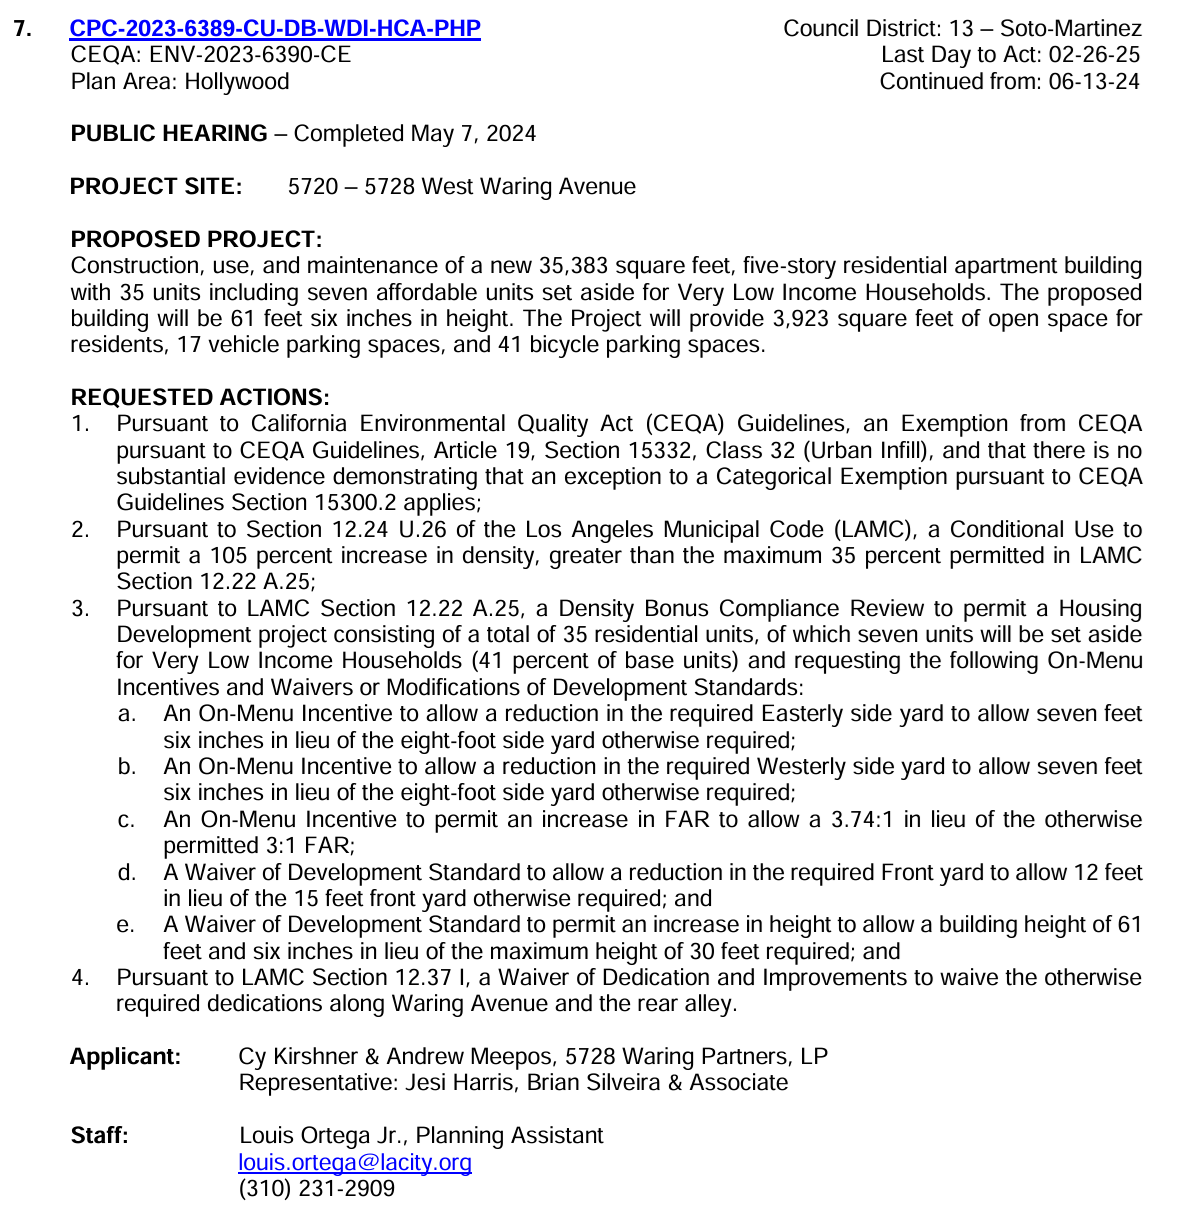
\includegraphics[width=\textwidth]{figures/example-agenda-item.png}
}
\end{center}
\end{figure}

\pagebreak

%%%%%%%%%%%%%%%%%%%%%%%%%%%%%%%%%%%%%%%%%%%%%%
\begin{figure}[H]
\caption{Example of a Minutes Item} \label{fig_example_minutes_item}
\vspace{-0.5cm}
\begin{center}
\fbox{
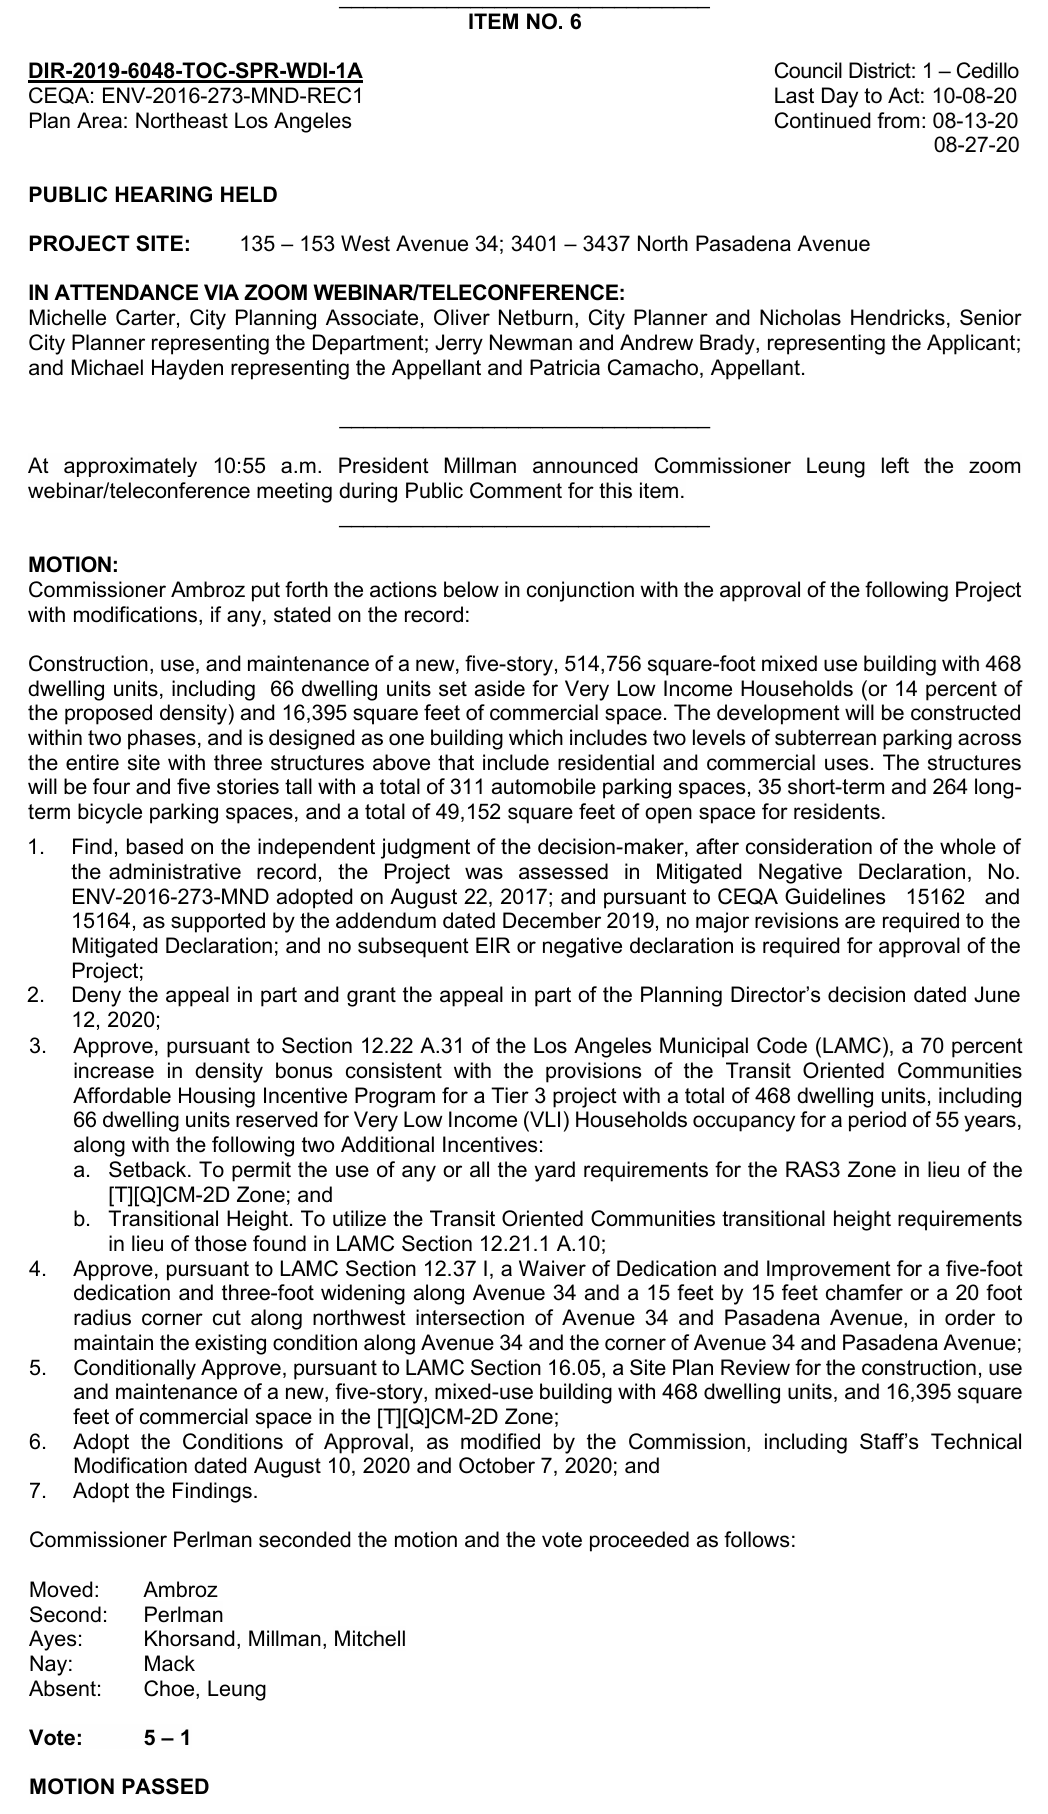
\includegraphics[height=0.95\textheight]{figures/example-minutes-item.png}
}
\end{center}
\end{figure}

\pagebreak

%%%%%%%%%%%%%%%%%%%%%%%%%%%%%%%%%%%%%%%%%%%%%%
\begin{figure}[H]
\caption{Example of a Support Letter} \label{fig_example_support_letter}
\vspace{-0.5cm}
\begin{center}
\fbox{
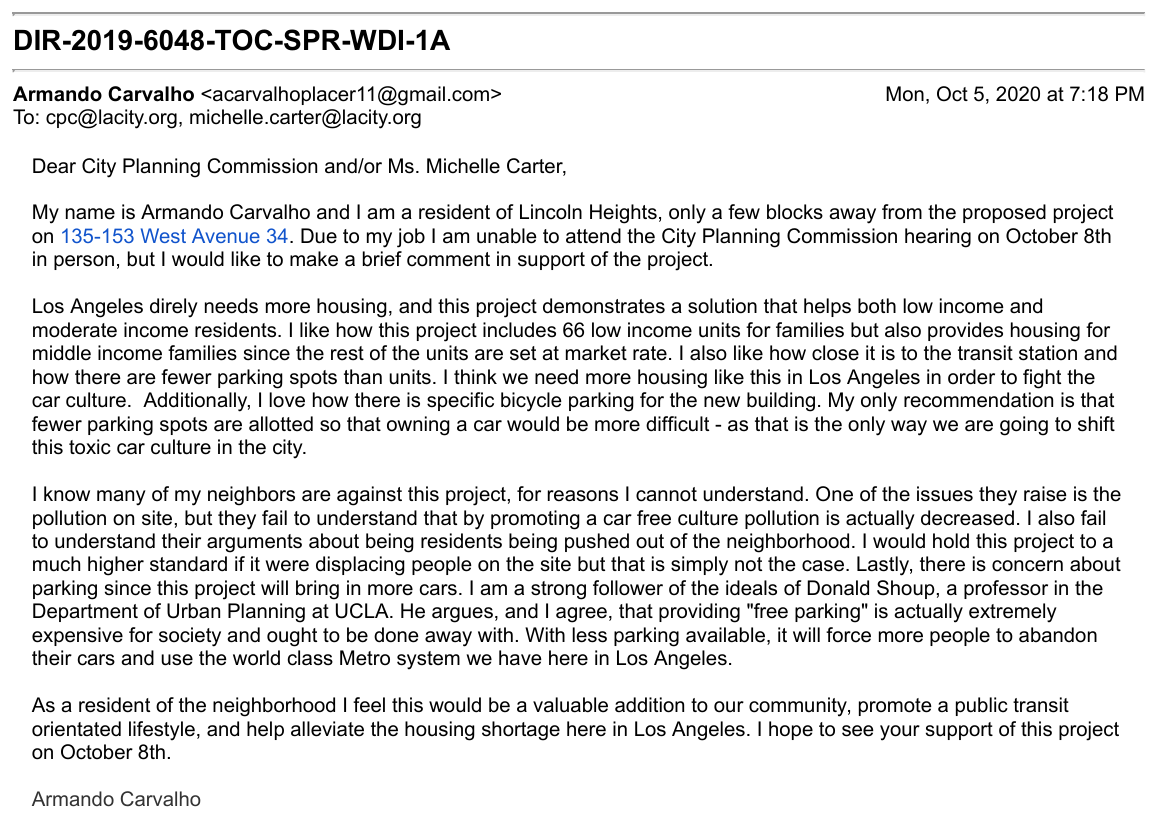
\includegraphics[width=\textwidth]{figures/example-support-letter.png}
}
\end{center}
\end{figure}

\pagebreak

%%%%%%%%%%%%%%%%%%%%%%%%%%%%%%%%%%%%%%%%%%%%%%
\begin{figure}[H]
\caption{Example of an Oppose Letter} \label{fig_example_oppose_letter}
\vspace{-0.5cm}
\begin{center}
\fbox{
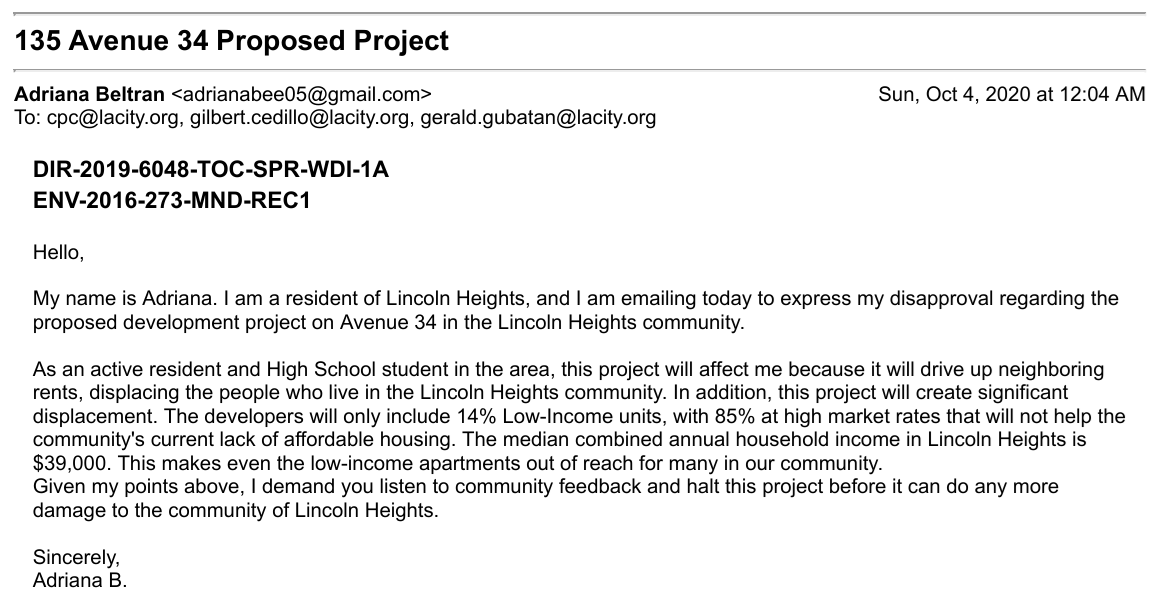
\includegraphics[width=\textwidth]{figures/example-oppose-letter.png}
}
\end{center}
\end{figure}

\pagebreak

%%%%%%%%%%%%%%%%%%%%%%%%%%%%%%%%%%%%%%%%%%%%%%
\begin{figure}[H]
\caption{Scree Plot of PCA Components} \label{fig_scree_plot}
\vspace{-0.5cm}
\begin{center}
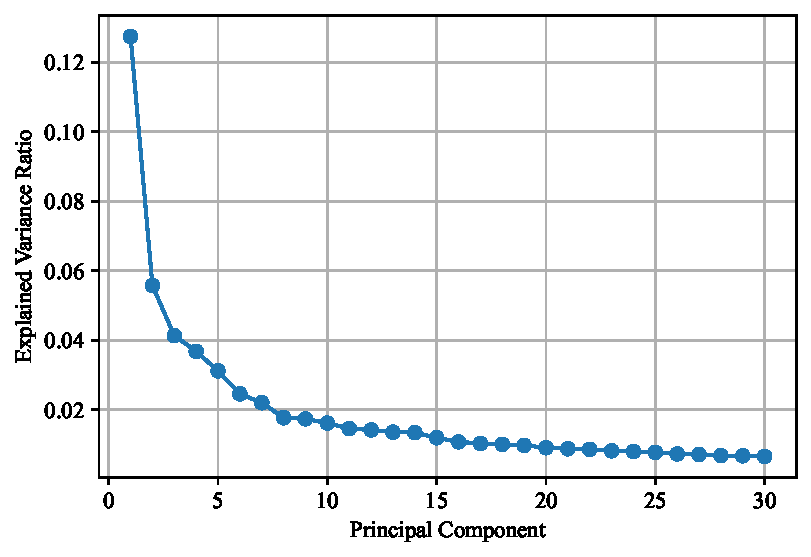
\includegraphics[width=\textwidth]{figures/fig_scree_plot.pdf}
\end{center}
\end{figure}

\pagebreak


%%%%%%%%%%%%%%%%%%%%%%%%%%%%%%%%%%%%%%%%%%%%%%
\begin{figure}[H]
\caption{PCA Reduced Embeddings with K-Means Clustering} \label{fig_clusters}
\vspace{-0.5cm}
\begin{center}
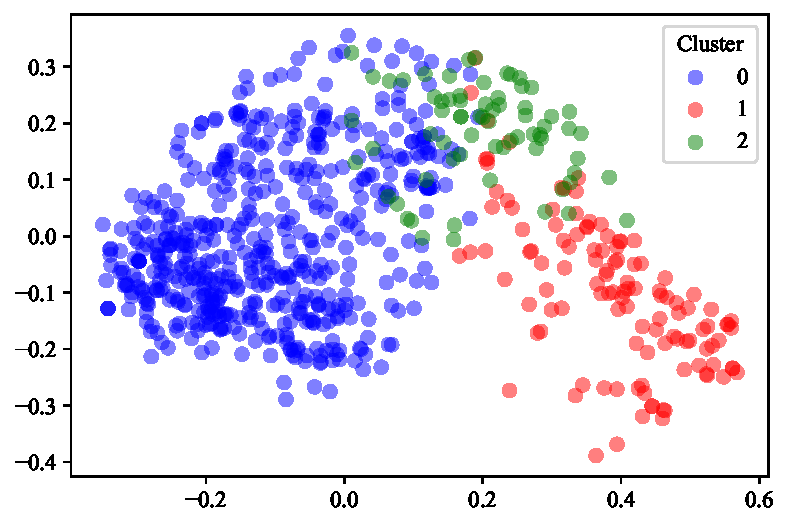
\includegraphics[width=\textwidth]{figures/fig_clusters.pdf}
\end{center}
\end{figure}

\pagebreak

%%%%%%%%%%%%%%%%%%%%%%%%%%%%%%%%%%%%%%%%%%%%%%
\begin{figure}[H]
\caption{Distribution of Number of Support and Opposition Letters} \label{fig_support_oppose}
\vspace{-0.5cm}
\begin{center}
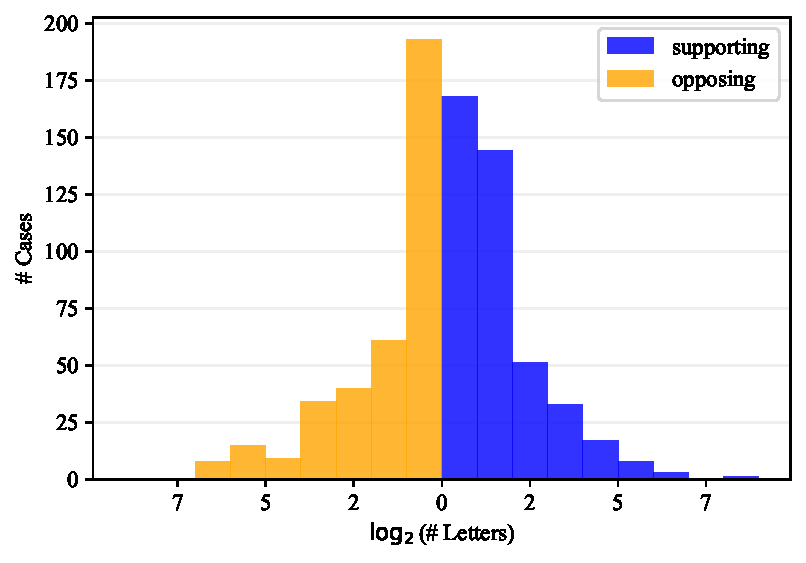
\includegraphics[width=\textwidth]{figures/fig_support_oppose.pdf}
\end{center}
\end{figure}

\pagebreak


%%%%%%%%%%%%%%%%%%%%%%%%%%%%%%%%%%%%%%%%%%%%%%
\begin{table}[H]
\caption{Summary of Motion Outcomes and Vote Results}
\vspace{0.2cm}
\label{tab_result_unanimity}
\begin{adjustbox}{max width=\textwidth}
\begin{threeparttable}
\begin{tabular}{lrrrrr} \toprule
 & \multicolumn{3}{c}{Unanimity} &  & \\ \cline{2-4} 
 & Unanimous & 1 Nay & >1 Nays & \multicolumn{2}{c}{Total} \\ \midrule
\textit{Project Implication} & & & & & \\ 
~ ~ APPROVED & 365 & 23 & 4 & 392 & (53.9\%) \\ [1ex] 
~ ~ APPROVED IN PART OR WITH MODIFICATIONS & 183 & 17 & 16 & 216 & (29.7\%) \\ [1ex] 
~ ~ DELIBERATIONS CONTINUED TO FUTURE DATE & 108 & 4 & 0 & 112 & (15.4\%) \\ [1ex] 
~ ~ DENIED & 5 & 0 & 2 & 7 & (1.0\%) \\ [1ex] 
~ ~ TOTAL & 661 & 44 & 22 & 727 &  \\ [1ex] 
 & (90.9\%) & (6.1\%) & (3.0\%) &  &  \\ [1ex] 
\end{tabular}

\begin{tablenotes}

\item {\textit{Notes: } This table shows the number of cases decided on by the City Planning Commission, organized by the implication of the motion for the project proposal and the unanimity of the vote.}
\end{tablenotes}
\end{threeparttable}
\end{adjustbox}
\end{table}

\pagebreak

\begin{table}[H]
  \centering
  \caption{Ordered Logit Regression Results}
  \vspace{0.2cm}
  \label{tab_ologit_results}
  \begin{adjustbox}{max width=\textwidth}
    \begin{threeparttable}
      \centering
      \begin{tabular}{lcccc}
\toprule
 & (1) & (2) & (3) & (4) \\
\midrule
 &  &  &  &  \\
Semantic Uniqueness & -0.325*** & -0.258*** & -0.259*** & -0.228** \\
 & (0.080) & (0.083) & (0.088) & (0.105) \\
 &  &  &  &  \\
Agenda Perplexity &  & -4.649 & -3.548 & -3.861 \\
 &  & (3.209) & (3.197) & (3.250) \\
 &  &  &  &  \\
Agenda Order &  & 0.095* & 0.086* & 0.042 \\
 &  & (0.050) & (0.050) & (0.053) \\
 &  &  &  &  \\
No. Agenda Items &  & -0.053 & -0.041 & -0.013 \\
 &  & (0.044) & (0.044) & (0.046) \\
 &  &  &  &  \\
Consent Calendar &  & 1.456*** & 1.357*** & 1.423*** \\
 &  & (0.279) & (0.292) & (0.304) \\
 &  &  &  &  \\
$\log_2$(\# Support) &  & 0.038 & 0.049 & 0.051 \\
 &  & (0.055) & (0.058) & (0.057) \\
 &  &  &  &  \\
$\log_2$(\# Oppose) &  & -0.169*** & -0.195*** & -0.209*** \\
 &  & (0.054) & (0.058) & (0.059) \\
 &  &  &  &  \\
Semantic Cluster FE & N & Y & Y & Y \\
 &  &  &  &  \\
Council District FE & N & N & Y & Y \\
 &  &  &  &  \\
Suffix Group FE & N & N & N & Y \\
 &  &  &  &  \\
$\mu_0$ & -2.641*** & -7.425** & -6.324* & -6.248* \\
 & (0.271) & (3.516) & (3.520) & (3.563) \\
 &  &  &  &  \\
$\mu_1$ & -1.136*** & -5.844* & -4.696 & -4.556 \\
 & (0.253) & (3.504) & (3.505) & (3.549) \\
 &  &  &  &  \\
No. of Obs & 727 & 727 & 727 & 727 \\
Pseudo R2 & 0.013 & 0.049 & 0.068 & 0.090 \\
\bottomrule
\end{tabular}

        \begin{tablenotes}[flushleft]
        \footnotesize
        \item Robust standard errors in parentheses. * $p<0.1$, ** $p<0.05$, *** $p<0.01$.
        \item \textit{Notes:} This table reports coefficient estimates from the ordered logit regression 
        described in Section \ref{sec_methodology}.
      \end{tablenotes}
    \end{threeparttable}
  \end{adjustbox}
\end{table}

\pagebreak

\begin{table}[H]
  \centering
  \caption{Ordered Logit Marginal Effects}
  \label{tab_ologit_marginal_effects}
  \begin{adjustbox}{max width=\textwidth}
    \begin{threeparttable}
      \begin{tabular}{lccc}
\toprule
                  &       (1) &       (2) &       (3) \\
\midrule
                  & Outcome 2 & Outcome 1 & Outcome 0 \\
                  &           &           &           \\
         Distance &   -0.048* &    0.020* &    0.028* \\
                  &   (0.022) &   (0.009) &   (0.013) \\
                  &           &           &           \\
Agenda Perplexity &    -0.819 &     0.345 &     0.474 \\
                  &   (0.687) &   (0.294) &   (0.396) \\
                  &           &           &           \\
     Agenda Order &     0.009 &    -0.004 &    -0.005 \\
                  &   (0.011) &   (0.005) &   (0.006) \\
                  &           &           &           \\
 No. Agenda Items &    -0.003 &     0.001 &     0.002 \\
                  &   (0.010) &   (0.004) &   (0.006) \\
                  &           &           &           \\
 Consent Calendar &  0.302*** & -0.127*** & -0.175*** \\
                  &   (0.062) &   (0.026) &   (0.039) \\
                  &           &           &           \\
      No. Support &     0.011 &    -0.005 &    -0.006 \\
                  &   (0.012) &   (0.005) &   (0.007) \\
                  &           &           &           \\
       No. Oppose & -0.044*** &  0.019*** &  0.026*** \\
                  &   (0.012) &   (0.005) &   (0.007) \\
                  &           &           &           \\
  Cluster Effects &         y &         y &         y \\
                  &           &           &           \\
 District Effects &         y &         y &         y \\
                  &           &           &           \\
   Suffix Effects &         y &         y &         y \\
                  &           &           &           \\
       No. of Obs &       727 &       727 &       727 \\
\bottomrule
\end{tabular}

        \begin{tablenotes}[flushleft]\footnotesize
            \item[] \parbox[t]{\linewidth}{%
            Robust standard errors in parentheses.
            * $p<0.1$, ** $p<0.05$, *** $p<0.01$.}
        \item \textit{Notes:} This table reports estimated marginal effects from the ordered logit regression 
        in column (4) of Table \ref{tab_ologit_results}.
      \end{tablenotes}
    \end{threeparttable}
  \end{adjustbox}
\end{table}


\pagebreak

\pagebreak

\pagebreak

\appendix

\renewcommand{\thefigure}{\thesection\arabic{figure}}
\renewcommand{\thetable}{\thesection\arabic{table}}

\makeatletter
\@addtoreset{figure}{section}
\@addtoreset{table}{section}
\makeatother

\section{Data Appendix} \label{sec_data_appendix}

\subsection{Data Extraction with LLMs}

Extracting data from the raw PDFs downloaded from the Planning Department website is a multi-step process. First, individual agenda items need to be extracted from the raw agenda PDF. This is difficult using traditional NLP methods because the boundaries between agenda items in the PDF are not always consistently demarcated. However, LLMs are quite suited to this task of identifying the unique agenda items out of a single PDF containing the agenda.

The first step, therefore, is to extract the individual agenda items. Figure \ref{fig_split_agenda_prompt} shows the prompt we used to have the LLM read the agenda, then extract each individual agenda item. We ask the LLM to return the agenda's item number, its title (which is a Planning Department case number for any items requiring a decision), and a short summary of the agenda item.

After the agenda items are extracted, the next step is to extract data about each agenda item, using the agenda text. The raw agenda PDF is split into its individual components based on the extracted item number and title for each agenda item. The text for each individual agenda item is then fed into the prompt shown in Figure \ref{fig_agenda_items_prompt}. The outputted response is then used to extract the data features listed in Section \ref{sec_data}.

After extracting data from the agenda text, we extract information about the deliberations over each agenda item from the minutes text. We first split the minutes PDF into the components relevant to each individual item, using the item number and title. We then take the agenda text for that item and the minutes text for that item and feed it into the prompt shown in Figure \ref{fig_minutes_prompt}. The response from the LLM is then processed to extract the data features.

Lastly, we 



\pagebreak

\begin{figure}[H]
\caption{Prompt to Split and Summarize Agenda} \label{fig_split_agenda_prompt}
\vspace{-0.5cm}
\begin{center}
\fbox{
\begin{minipage}{\textwidth}
\texttt{
\footnotesize
The following extracted PDF text contains the agenda for a LA City Planning Commission meeting. \\ 
\\ 
For each agenda item, return a summary in the following format:\\ 
\\ 
ITEM NO: <agenda item number>\\ 
TITLE: <title of agenda item>\\ 
SUMMARY: <short summary of agenda item>\\ 
\\ 
Separate each response by "------"\\ 
\\ 
AGENDA:\\ 
\\ 
[AGENDA TEXT]
}
\end{minipage}
}
\end{center}
\end{figure}

\pagebreak

\begin{figure}[H]
\caption{Prompt to Extract Agenda Item Data} \label{fig_agenda_items_prompt}
\vspace{-0.6cm}
\begin{center}
\fbox{
\begin{minipage}{\textwidth}
\texttt{
\footnotesize
--- AGENDA ITEM ----\\ 
\\ 
<<agenda item text>>\\ 
\\ 
--- PROMPT ----\\ 
\\ 
The document above is an agenda item from a Los Angeles City Planning Commission (CPC) meeting.\\ 
\\ 
Please return a response in the following format:\\ 
\\ 
---- YOUR RESPONSE FORMAT ----\\ 
RELATED CASES:\\ 
<A comma separated list of relevant planning department case numbers>\\ 
\\ 
COUNCIL DISTRICT:\\ 
<What council district is the project located in? Your only options are: 1, 2, 3, 4, 5, 6, 7, 8, 9, 10, 11, 12, 13, 14, 15, CITYWIDE>\\ 
\\ 
COUNCIL MEMBER:\\ 
<Who is the council member representing that district? If district is CITYWIDE, say N/A>\\ 
\\ 
LAST DAY TO ACT:\\ 
<What is the last day to act? Format your answer as YYYY-MM-DD>\\ 
\\ 
SUMMARY OF PROJECT:\\ 
<Summarize the project and the requested actions.>\\ 
\\ 
RELEVANT LAWS:\\ 
<List any referenced legal codes, ordinances, or programs that apply to the requested actions>\\ 
\\ 
APPEALED:\\ 
<Was there an appeal against an earlier determination? Say YES or NO>\\ 
\\ 
SUMMARY OF APPEAL:\\ 
<Summarize the appeal if there was one. If no appeal, say N/A>\\ 
\\ 
DISPUTED LAWS:\\ 
<List the referenced legal codes, ordinances, or programs which are in dispute based on the appeal. If no appeal, say N/A>
}
\end{minipage}
}
\end{center}
\end{figure}

\pagebreak

\begin{figure}[H]
\caption{Prompt to Extract Data from Minutes} \label{fig_minutes_prompt}
\vspace{-0.6cm}
\begin{center}
\fbox{
\begin{minipage}{\textwidth}
\texttt{
\footnotesize
--- AGENDA ITEM ----\\ 
\\ 
<<agenda item text>>\\ 
\\ 
--- MINUTES OF DISCUSSION ----\\ 
\\ 
<<minutes text for item>>\\ 
\\ 
--- PROMPT ----\\ 
\\ 
I just gave you two documents related to a Los Angeles City Planning Commission (CPC) hearing.\\ 
\\ 
The first document is the agenda item to be discussed, with requested actions.\\ 
\\ 
The second document is the minutes of the discussion, the proposed motion by the CPC, the votes on the motion by the CPC members, and whether the motion ultimately passed.\\ 
\\ 
Please return a response in the following format:\\ 
\\ 
---- YOUR RESPONSE FORMAT ----\\ 
RELATED CASES:\\ 
<A comma separated list of relevant planning department case numbers>\\ 
\\ 
SUMMARY OF AGENDA ITEM:\\ 
<A summary of the agenda item to be discussed>\\ 
\\ 
SUMMARY OF CPC DELIBERATIONS:\\ 
<A summary of the deliberations of the CPC.>\\ 
\\ 
SUMMARY OF CPC MOTION:\\ 
<A summary of the motion voted on by the CPC>\\ 
\\ 
MOVED:\\ 
<Which commission member moved the motion? If multiple motions were made, use only the last motion. If no motion was made, say "N/A".>\\ 
\\ 
SECONDED:\\ 
<Which commission member seconded the motion? If multiple motions were made, use only the last motion. If no motion was made, say "N/A".>
}
\end{minipage}
}
\end{center}
\end{figure}

\pagebreak

\begin{figure}[H]\ContinuedFloat
\caption{Prompt to Extract Data from Minutes (cont'd)} \vspace{-0.6cm}
\begin{center}
\fbox{
\begin{minipage}{\textwidth}
\texttt{
\footnotesize
AYES:\\ 
<A comma separated list of commission members who voted for the motion. If multiple motions were made, use only the last motion. If no one voted for, say "NONE". If no motion was made, say "N/A".>\\ 
\\ 
NAYS:\\ 
<A comma separated list of commission members who voted against the motion. If multiple motions were made, use only the last motion. If no one voted against, say "NONE". If no motion was made, say "N/A".>\\ 
\\ 
ABSTAINED:\\ 
<A comma separated list of commission members who abstained from voting on the motion. If multiple motions were made, use only the last motion. If no one abstained, say "NONE". If no motion was made, say "N/A".>\\ 
\\ 
RECUSED:\\ 
<A comma separated list of commission members who were recused from voting on the motion. If multiple motions were made, use only the last motion. If no one was recused, say "NONE". If no motion was made, say "N/A".>\\ 
\\ 
ABSENT:\\ 
<A comma separated list of commission members who were absent. If multiple motions were made, use only the last motion. If no one was absent, say "NONE". If no motion was made, say "N/A".>\\ 
\\ 
VOTE RESULT:\\ 
<Did the motion pass or fail? Your only options are MOTION PASSED, MOTION FAILED, N/A>\\ 
\\ 
RESULT OF APPEAL:\\ 
<If the agenda item involved an appeal, say whether the appeal was granted or denied. Your only options are: APPEAL GRANTED, APPEAL GRANTED IN PART, APPEAL DENIED, NO APPEAL, DELIBERATIONS CONTINUED TO FUTURE DATE, APPLICATION WITHDRAWN>\\ 
\\ 
IMPLICATION FOR PROJECT:\\ 
<What is the implication of the vote for the original requested actions? Your only options are: APPROVED, APPROVED IN PART OR WITH MODIFICATIONS, DENIED, DELIBERATIONS CONTINUED TO FUTURE DATE, APPLICATION WITHDRAWN>
}
\end{minipage}
}
\end{center}
\end{figure}

\pagebreak

\begin{figure}[H]
\caption{Prompt to Extract Data from Supplemental Documents} \label{fig_supplemental_docs_prompt}
\vspace{-0.6cm}
\begin{center}
\fbox{
\begin{minipage}{\textwidth}
\texttt{
\footnotesize
==== LIST OF AGENDA ITEMS ====\\ 
\\ 
<<full agenda text>>\\ 
\\ 
==== DOCUMENT ====\\ 
\\ 
<<document text>>\\ 
\\ 
==== PROMPT ====\\ 
\\ 
I just gave you a list of agenda items from a LA City Planning Commission meeting, followed by a document submitted to that meeting. \\ 
\\ 
Return a response in the following format:\\ 
\\ 
\\ 
==== YOUR RESPONSE FORMAT ====\\ 
\\ 
TYPE OF DOCUMENT:\\ 
<What type of document is it? Your only options are: LETTER OR PETITION, TECHNICAL MODIFICATION OR PROCEDURAL MATTER, SCIENTIFIC OR TECHNICAL REPORT, CV OR BIOGRAPHY, CORRUPTED/ILLEGIBLE/BLANK, TITLE OR SECTION HEADING, OTHER.>\\ 
\\ 
TYPE OF AUTHOR:\\ 
<What type of entity wrote the document? Your only options are: INDIVIDUAL, ADVOCACY GROUP, CONSULTANT, LAWYER, DEVELOPER, PUBLIC OFFICIAL, OTHER.>\\ 
\\ 
SUMMARY OF DOCUMENT:\\ 
<Summarize the contents of the document.>\\ 
\\ 
REFERENCED AGENDA ITEMS:\\ 
<List the agenda items, as a comma delimited list of item numbers, that the submitted document references or is relevant to. If none, say NONE.>\\ 
\\ 
SUPPORT OR OPPOSE:\\ 
<Does the submitted document support or oppose the referenced agenda items? Your only options are: DEFINITELY SUPPORT, SOMEWHAT SUPPORT, DEFINITELY OPPOSE, SOMEWHAT OPPOSE, NEUTRAL, NOT RELEVANT.>
}
\end{minipage}
}
\end{center}
\end{figure}


\end{document}

